\documentclass[12pt, a4paper]{article}
\usepackage[english]{babel}
\usepackage[utf8]{inputenc}
\usepackage{setspace}
\usepackage[bookmarksopen,colorlinks,linkcolor=black,urlcolor=Blue,citecolor=black]{hyperref}
\usepackage{multirow}
\usepackage{enumerate}
\usepackage{graphicx}
\usepackage{array}
\usepackage{caption}
\usepackage{float,lscape}
\usepackage{longtable}
\usepackage[margin=2.54cm, include foot]{geometry}
\usepackage{enumitem}
\usepackage{wrapfig}
\usepackage{threeparttable}
\usepackage{multicol}
\usepackage{dcolumn}
\usepackage{geometry}
\usepackage{makecell}
\usepackage{amsmath}
\usepackage[nameinlink]{cleveref}
\usepackage{appendix}
\usepackage{mathtools}
\usepackage{booktabs}
\usepackage{subcaption}
\usepackage[T1]{fontenc}
\usepackage{rotating}
\usepackage[natbibapa]{apacite}
\usepackage[usenames,dvipsnames]{color}
\usepackage{afterpage}
\usepackage{bbm}
\usepackage{pdflscape}
\hypersetup{
	colorlinks,
	citecolor=Blue,
	linkcolor=Blue,
	}
\usepackage{titling}
\usepackage{etoolbox}

% Toggle to display figures in-place (true) or at the end (false)
\newtoggle{figuresinplace}
%\toggletrue{figuresinplace} % Figures in place
\togglefalse{figuresinplace} % Figures at the end

%\onehalfspacing % Uncomment to turn on 1.5 spacing
%\doublespacing % Uncomment to turn on 2 spacing

\addto\extrasenglish{
    \def\sectionautorefname{Section}
}

\begin{document}
\renewcommand{\BOthers}[1]{et al.\hbox{}}
\newcommand\fnote[1]{\captionsetup{font=footnotesize}\caption*{#1}}

% FOR ADDING IN-LINE COMMENTS THAT CAN BE TOGGLED ON AND OFF
\newcommand{\xxx}[2][show]{ % Replace "show" with any other word to hide XXX comments.
 \ifthenelse{\equal{#1}{show} }{ \textcolor{red}{X #2 X}}{}}

%\vspace{-2.35cm}
\title{\Large \textbf{The impact of pension reforms on retirees' health}}
\author{Pablo Uribe \\ \small \textit{Yale University}} 
\maketitle
\thispagestyle{empty}
\vspace{-0.5cm}

% \begin{center}
%     \Large \textcolor{red}{This is a preliminary draft of an ongoing project. Please do not share}
% \end{center}

%%%%%%%%%%%%%%%%%%%%%%%%%%%%%%%%%%%%%%%%%%%%%%%%%%%%
\begin{abstract}
    
Lorem ipsum dolor sit amet, consectetur adipiscing elit, sed do eiusmod tempor incididunt ut labore et dolore magna aliqua. Ut enim ad minim veniam, quis nostrud exercitation ullamco laboris nisi ut aliquip ex ea commodo consequat. Duis aute irure dolor in reprehenderit in voluptate velit esse cillum dolore eu fugiat nulla pariatur. Excepteur sint occaecat cupidatat non proident, sunt in culpa qui officia deserunt mollit anim id est laborum.

\end{abstract}


\textit{\textbf{Keywords:}} Pay as You Go, Pension, Public Pension, Retirement Pension.

\vspace{0.5cm}
\textit{\textbf{JEL Classification:}} H55, J14, J26.

\vspace{.5cm}

\newpage
\setcounter{page}{1}
%%%%%%%%%%%%%%%%%%%%%%%%%%%%%%%%%%%%%%%%%%%%%%%%%%%%
\section{Introduction}

Pension reforms can have far-reaching consequences, affecting both labor market dynamics and individual well-being. As governments face increasing fiscal pressure from aging populations, raising the retirement age has become a common policy response. A large body of research shows that increasing the retirement age influences employment, earnings, and the timing of retirement \citep{geyer2020labor,hernaes2016pension,sanchez2014delaying,cribb2016signals,de2018social,geyer2021closing,rabate2020employment,atalay2015impact,staubli2013does,rabate2024increasing}. The majority of the evidence comes from papers looking at these policies in developed countries, where the effects on the employment rate range from 6.3 percentage points (pp) in the UK to 21.2 pp in the Netherlands. In line with this, \citet{pilipiec2021effect} show in a systematic review of the literature that there is a consensus on the positive effects of increasing the retirement age on labor force participation among older workers.

On the other hand, evidence on the health effects of working beyond the initial retirement age remains mixed —some studies suggest little to no impact \citep{hagen2018effects}, while others find adverse consequences \citep{coe2011retirement}. Overall, the evidence on the effects of these reforms on the well-being of older workers is scarce and inconclusive \citep{pilipiec2021effect}, with some studies showing positive effects of increasing the retirement age on workers' mental health \citep{maimaris2010impact}. However, most of the literature is concentrated in developed countries, with little to no studies focused on developing economies, particularly in Latin America. In particular, \citet{de2019trends} provide descriptive evidence on the health and retirement trends in this region to conclude that health is not a barrier to raising the retirement age. 

This paper leverages a pension reform in Colombia that increased the retirement age by two years. In 1993, Congress passed Law 100, which among other social security systems, created a dual-pillar pension system where individuals could choose between a public pay-as-you-go scheme and a private individual savings regime. The Law established the retirement age for people to be eligible for a pension if they were affiliated to the public system. It also specified that this age would be increased by two years in 2014. Interestingly, a transition regime was established within the Law, so that individuals who were at least 35 years old (women) or 40 years old (men) in December 23, 1994, or those who had accumulated 750 weeks of contributions by that date, were permitted to retire under the original age thresholds of 55 (women) and 60 (men) until 2014.

This transition regime was later modified by Legislative Act 01 of 2005, which accelerated its elimination by moving the 2014 deadline to July 31, 2010. This implies that women (men) who were part of the Law 100 transition regime and were born on or before July 31, 1955 (1950), would still be able to retire as expected. However, individuals born after this date --even if they were part of the transition regime-- would have to work for two more years beyond the original retirement age.

I leverage the birth date cutoff introduced by the Act to estimate the effects of increasing the retirement age on health outcomes for older workers using a regression discontinuity (RD) design. For that purpose, I use Colombian administrative data from the universe of formal workers who are close to retirement, and data from all health services demanded by these individuals between 2009 and 2022. This set of linked datasets allow me to track individuals' labor market outcomes and health claims over time.

To the best of my knowledge, this is the first paper to causally establish the impact of such reforms on individuals' health in a developing country. 

The rest of the paper is organized as follows. First, \autoref{sec:setting} provides details on the Colombian pension system and Legislative Act 01 of 2005. \autoref{sec:data} describes the main datasets along with their sources, showing descriptive statistics for the main sample. \autoref{sec:strategy} outlines the empirical strategy used to estimate the causal effects of the reform, and \autoref{sec:results} presents the results. Finally, \autoref{sec:conclusion} concludes. 



%%%%%%%%%%%%%%%%%%%%%%%%%%%%%%%%%%%%%%%%%%%%%%%%%%%%%
\section{Setting \label{sec:setting}}

Law 100 of 1993 established Colombia’s Social Security System, which is made up of three subsystems: pensions, health, and professional risks. The General Pension System (SGP, by its Spanish acronym) created a dual-pillar structure that allows workers to choose between a public pay-as-you-go scheme and an individual savings regime. Once workers select a regime, they are legally required to stay affiliated to the same one for a minimum of five years before transferring. The main objective of this new system was to expand pension coverage across the country and to make sure people were covered against any contingencies that may derive from old age, disabilities or death.

Regardless of the system that an individual chooses to join when starting their work life, contributions are handled equivalently. For dependent workers, the contribution is split between employers and employees, with the former covering a larger share of the total contribution. On the other hand, independent workers are responsible to pay for the entirety of their contribution. While the share of income that has to be contributed is the same for everyone, independent workers calculate this share on 40\% of their total salary instead ---since they have to cover it in its entirety. Currently, the mandatory contribution is 16\% of the monthly wage. For dependent workers, employers cover 12\% and the worker covers the remaining 4\%.

\subsection{The Private Pension Regime}

The \textit{Régimen de Ahorro Individual Solidario} (RAIS) --or Individual Savings Regime with Solidarity-- operates as a fully funded scheme where each worker accumulates savings in a private pension account. These pensions are managed by private funds who charge administration fees and are responsible for investing the money. Each worker can choose the fund that suits their needs and providers typically offer different investment portfolios depending on individuals' risk tolerance. Since contributors have flexibility to switch between providers, the latter have to compete to attract individuals.

A key feature of this regime is that there is no fixed retirement age. Instead, pension eligibility depends on the accumulated balance being sufficient to finance a monthly lifetime pension of at least 110\% of the monthly minimum wage. If the individual wants to keep contributing towards their pension, their employer is required to continue paying their share of the contribution while there still exists a contract with the employer until the latter turns 60 (women) or 62 (men).

Alternatively, if savings are not enough to finance such pension, workers can obtain a guaranteed minimum pension as long as they have contributed for at least 1,150 weeks. However, if an individual fails to meet the pension requirements, they receive a lump-sum payment upon retirement, which includes the total amount they contributed and the returns on the investment. 

\subsection{The Public Pension Regime}
The \textit{Régimen de Prima Media} (RPM) --or Average Premium Regime-- is Colombia's public pay-as-you-go pension system. Under this scheme, contributions from active workers finance the pensions of current retirees. Unlike the private system, where pension is determined by the accumulated contributions plus market returns, the RPM guarantees a fixed pension formula, making it the preferred option for workers seeking stability in their old age.

Colpensiones currently serves as the administrator of this public pension system. Originally, the administration of the RPM was the responsibility of the \textit{Instituto de Seguros Sociales} (ISS); however, subsequent institutional reforms led to Colpensiones taking over these functions to provide a more focused and efficient management of resources. In this way, Colpensiones continues the work of the ISS to ensure that the benefit structure of the RPM is preserved.

Law 100 of 1993 initially set the retirement age at 55 years for women and 60 years for men, with a requirement of 1,000 weeks of contributions to qualify for a pension. Pension amounts are determined by a replacement rate that depends on total weeks contributed, with a minimum pension floor set at the legal monthly minimum wage. The calculated rate is applied to the average monthly salary of the last 10 years of contributions to determine the total allowance that will be paid monthly to the retiree.\footnote{A total of 13 allowances are paid over the course of a year, since retirees receive a bonus payment on top of the monthly pension in December.} In addition to the standard old-age pension, the system provides disability and survivor benefits, ensuring coverage for individuals who experience a loss of labor capacity or for the dependents of deceased workers.

A key feature of the RPM, as established by Law 100, was the planned increase in the retirement age. The legislation established that, starting in 2014, the minimum retirement age would increase to 57 years for women and 62 years for men. This policy change was intended to improve the system’s financial sustainability by reducing the number of years individuals receive benefits while extending their contribution period. However, the Law also contemplated a Transition Regime (TR) that allowed certain workers to remain under the previous retirement conditions. Specifically, individuals who were at least 35 years old (women) or 40 years old (men) in December 23, 1994, or those who had accumulated 750 weeks of contributions by that date, were permitted to retire under the original age thresholds of 55 and 60. This transition regime created a gradual adjustment for those close to retirement while fully enforcing the new retirement age for younger cohorts.

However, these TR conditions were revised in subsequent reforms, further modifying the timeline for retirement eligibility and introducing additional constraints on early retirement. In its core, the system's structure was not heavily modified until Law 2381 of 2024. Since July 1, 2025, every formal worker has to be affiliated to Colpensiones with contributions up to 2.3 monthly minimum wages. If their income is higher, they may voluntarily choose the fund of their choice (Colpensiones or any private fund) to contribute on the rest of their income above the threshold.

\subsection{Legislative Act 01 of 2005 \label{subsec:la01}}

Legislative Act 01 of 2005 (LA-01) introduced a major reform to Colombia’s public pension system, accelerating the elimination of the transition regime established by Law 100 and further restricting early retirement options.\footnote{This reform only affects Colpensiones affiliates, as there is no age requirement for individuals contributing to RAIS.} Initially, the TR was set to expire in 2014, but LA-01 moved this deadline forward to July 31, 2010, except for individuals who had contributed to Colpensiones for at least 750 weeks --around 15 years-- by the time this Act came into force in July 25, 2005. These individuals maintained their status until 2014.

Maintaining this transition regime until July 31, 2010 implies that women (men) who were part of the TR as established by Law 100, would be able to retire at 55 (60) years old only if they were born on or before July 31, 1955 (1950). If an individual was originally part of the TR but was born on August 1, or later, they would not be able to retire as expected and would have to work an additional two years, unless they met the contribution requirement in 2005. For those who met this requirement, they had until the end of 2014 to meet all the requirements and become entitled to a pension. Otherwise, they would have to work until they are 57 (women) or 62 (men) years old.



%%%%%%%%%%%%%%%%%%%%%%%%%%%%%%%%%%%%%%%%%%%%%%%%%%
\section{Data \label{sec:data}}

I use administrative data from several sources.\footnote{Details on data construction can be found in \autoref{sec:appdata}.} First, I use the Ministry of Health's \textit{Planilla Integrada de Liquidación de Aportes} (PILA). This dataset includes the entire population of formal workers in Colombia between 2008 and 2022. This is especially relevant since every social security contribution in the country has to go through PILA, so I am effectively seeing all individuals contributing towards their pension. Since the scope of this paper is to study the effects of a pension reform, I focus on a specific subset of the population. That is, all women born between 1953 and 1961, and all men born between 1948 and 1956. These dates are chosen so that I can see people born up to two years before and after the birth date cutoffs affected by LA-01. This is what I refer to as the master sample, and contains a total of \xxx{N} individuals. As explained in \autoref{subsec:la01}, LA-01 implicitly introduced a July 31 cutoff for men born in 1950 and women born in 1955. For the rest of the paper, I will refer to the male cohort as M50, and the female cohort as F55.

PILA provides comprehensive monthly information on individuals' contributions to pensions, healthcare, and occupational risk insurance. It includes detailed identifiers such as personal identification numbers, gender, and birth dates, along with extensive employment information, including wages, days worked, and employer characteristics for all formally employed workers in Colombia. I merge the master sample to these monthly records to track labor market outcomes for the individuals affected by the reform. For each of them, I have information on the real monthly wage (base 2018), and the pension fund they are affiliated to.

Second, I use the Ministry of Health's \textit{Registros Individuales de Prestación de Servicios de Salud} (RIPS). These records contain all health claims in the country, so I am able to track every consultation, procedure, emergency room visit, and hospitalization at the individual level. This dataset contains individual's identifications and the diagnosis code that identifies the specific pathology for which the user is demanding the service. These codes are assigned by a healthcare professional following the International Classification of Diseases ICD-10 \citep{icd10}. Since RIPS is available between 2009 and 2022, I am able to see the medical history for the master sample in that time period. This allows me to record the number and types of services demanded, the types of physicians consulted, and whether an individual suffered from a specific disease at a given point in time. Since these data have low incidence, I collapse the dataset at a yearly level.\footnote{More details on variable construction and data processing can be found in \autoref{sec:appdata}.}

Finally, in order to look at baseline balance around the birth date cutoffs introduced by LA-01, I use the 2005 Colombian census microdata. While I cannot directly match this dataset with the master sample, census data contain each individual's date of birth, so I use it as a secondary data source to look for any differences between those born before or after the cutoffs. The questionnaire includes a set of questions for whether the individual has had some illness in the past year, whether they work, are affiliated to a pension fund, and their educational attainment. 


\subsection{Summary Statistics}
The summary statistics for the master sample are shown in \xxx{Tabla}. Panel A shows labor market outcomes (wages, percent in Colpensiones, average pension contribution, dependents vs self-employed). Panel B shows health-related outcomes (number of services, diseases...).


%%%%%%%%%%%%%%%%%%%%%%%%%%%%%%%%%%%%%%%%%%%%%%%%%
\section{Empirical Strategy \label{sec:strategy}}

To understand the causal effect of the reform on retirees' health, I leverage the implementation of LA-01 and the clear cutoffs it introduced to implement a regression discontinuity design. I estimate a regression of the following form:

\begin{equation}
    Y_{ij} = \alpha_j + \delta_j f(Z_{i}) + \beta T_i + \gamma_i (f(Z_i)*T_i) + \varepsilon_i
\end{equation}

\noindent where $Y_{ij}$ is a specific labor market or health outcome of individual \textit{i}, who is a part of cohort \textit{j}. $f(.)$ is a function of the running variable $Z_i$. The latter represents the distance in weeks between the week of birth of individual \textit{i} and the cutoff that applies to cohort \textit{j}. This variable is standardized around the cutoffs, taking a value of zero when an individual is born on the same week as the cutoff that applies to them. For values of the running variable greater than zero, the indicator $T_i$ takes a value of one, implying that those individuals will lose their transition regime status and will have to work for an additional two years before becoming entitled for a pension. Finally, $\varepsilon_i$ is the error term.

The coefficient of interest is $\beta$, which captures the causal effect of increasing the retirement age by two years on the outcome of interest as long as the continuity assumption holds. That is, individuals should not be sorting on the running variable. If this holds, observations around the cutoff are expected to be as-good-as-randomly assigned to treatment, so there should be no observable statistical differences between those just above and below the cutoff. However, this relies on the number of observations around it, as there is a trade-off between bias and variance. A larger bandwidth means a higher number of observations, which reduces the variance and yields more precise estimates, but introduces bias as the relationship between the running variable and the outcomes is not as smooth the further they get from the cutoff. To minimize this trade-off, I choose an optimal bandwidth for each regression following \citet{calonico2014robust}, and \citet{calonico2020optimal}.

In the following subsections I will provide evidence that there is no manipulation and that the sample is balanced at baseline.


\subsection{Manipulation}
As previously described, the RD design relies on the continuity of the running variable around the cutoff point (i.e., that there are no ``jumps'' in the birth dates). If individuals know what the cutoff is, they could try to sort on the running variable to be eligible for the treatment. In this particular case, since the cutoff is defined by the individuals' birth dates and these are not explicitly mentioned in the Law, there is virtually no room for manipulation. To formally test this, I look at the distribution of birth dates by cohort and run a manipulation test following \citet{mccrary2008manipulation}. \autoref{fig:manipulation} shows the distributions of birth dates for men and women, along with the p-value from the manipulation test. There is an upward trend in birth dates consistent with an increase in population. Consistent with the fact that an individual cannot manipulate its own birth date, the p-values confirm that there is no sorting on the running variable for any of the samples (\xxx{$p=$ for men, and $p=$ for women}).

\iftoggle{figuresinplace}{
\begin{figure}[H]
\centering
\caption{Running variable distribution by cohort}\label{fig:manipulation}
\begin{subfigure}{.5\textwidth}
  \centering
  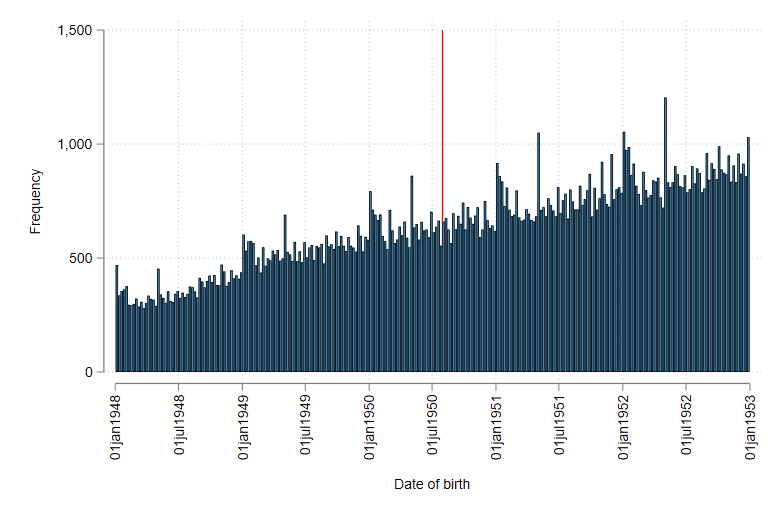
\includegraphics[width=\linewidth]{Graphs/hist_M50.png}
  \caption{M50 cohort}
\end{subfigure}%
\begin{subfigure}{.5\textwidth}
  \centering
  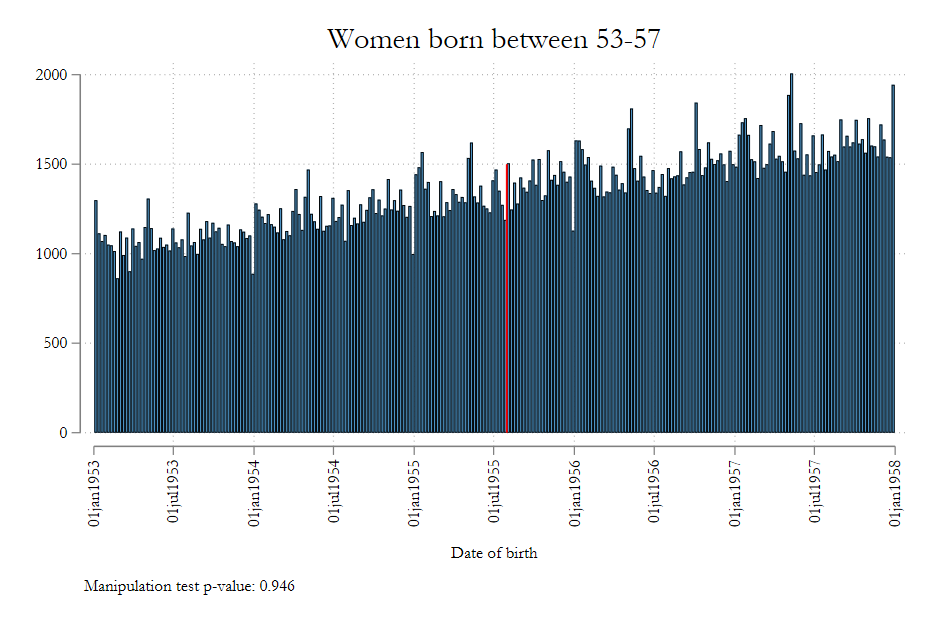
\includegraphics[width=\linewidth]{Graphs/hist_F55.png}
  \caption{F55 cohort}
\end{subfigure}
\fnote{\textit{Notes:} Panel (a) shows the distribution of birth dates for men born between 1948 and 1952. Panel (b) shows the distribution of birth dates for women born between 1953 and 1957. The red lines in each panel represent the cutoff date from LA-01. P-values from the McCrary density test are shown in the top left corner of each plot.}
\end{figure}
}{}


\subsection{Balance}

Another way to look at the plausibility of the continuity assumption is to compare individuals around the cutoff point in observable pre-treatment characteristics. For the design to be valid, there should not be any discontinuity in the average covariate values --i.e., treatment and control groups should be balanced. \autoref{fig:balance} suggests there is balance in relevant pre-treatment covariates from the 2005 Colombian census.\footnote{The 1993 census could also be used as a baseline measure, but it only contains individuals' ages (not their specific birth dates) so there is no way to construct a running variable.} There are no statistically significant differences in health outcomes as reported in the census between those who were born around the cutoff. Additionally, I see no evidence of discontinuities for relevant variables like being affiliated to a pension fund or being employed. This suggests that any impacts I find in my analysis are driven by LA-01, and are not explained by pre-treatment differences across treatment groups.

\iftoggle{figuresinplace}{
\begin{figure}[H]
\caption{Sample balance across cohorts}\label{fig:balance}
\centering 
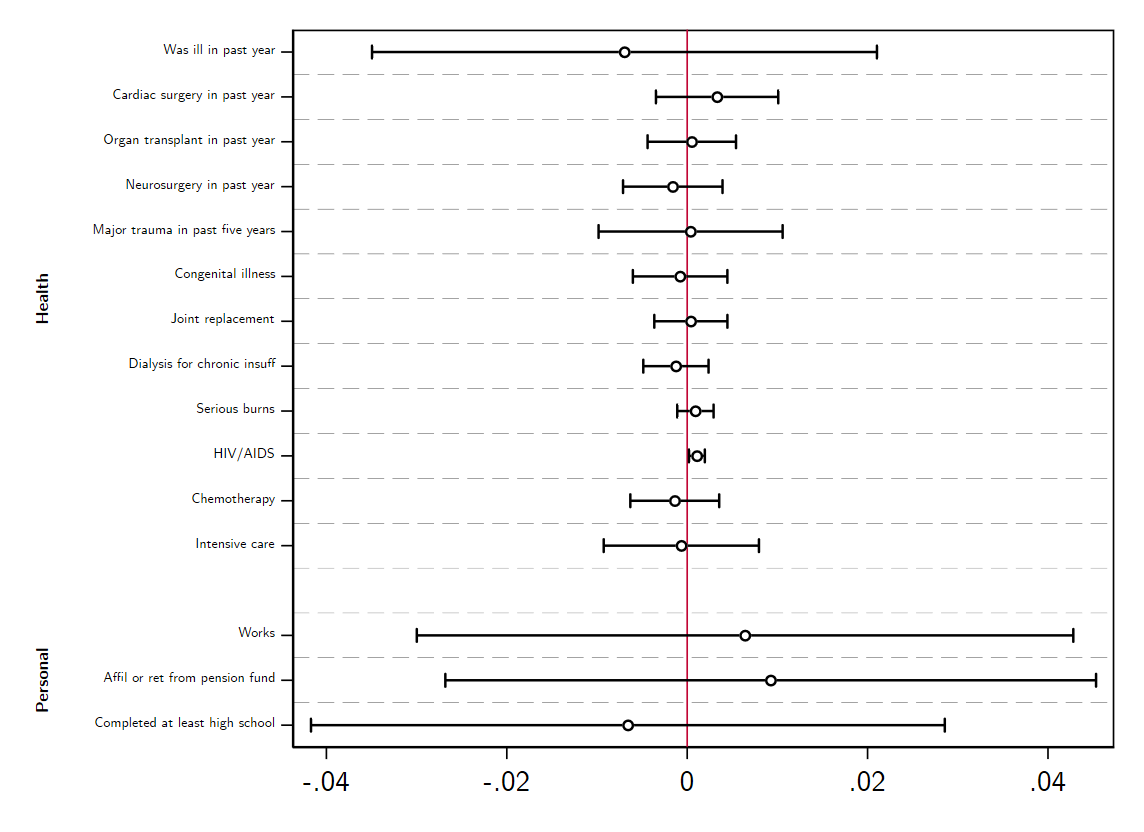
\includegraphics[width=\textwidth]{Graphs/balance_RD_final.png}
\fnote{\textit{Notes:} Each dot represents the point estimate from the RD regression. The lines across the coefficients are confidence intervals at the 95\% level.}
\end{figure}
}{}

%%%%%%%%%%%%%%%%%%%%%%%%%%%%%%%%%%%%%%%%%%%%%%%%%
\section{Results \label{sec:results}}



%%%%%%%%%%%%%%%%%%%%%%%%%%%%%%%%%%%%%%%%%%%%%%%%%
\section{Conclusions \label{sec:conclusion}}

\newpage

\iftoggle{figuresinplace}{}{
\section*{Figures}

\begin{figure}[H]
\centering
\caption{Running variable distribution by cohort}\label{fig:manipulation}
\begin{subfigure}{.5\textwidth}
  \centering
  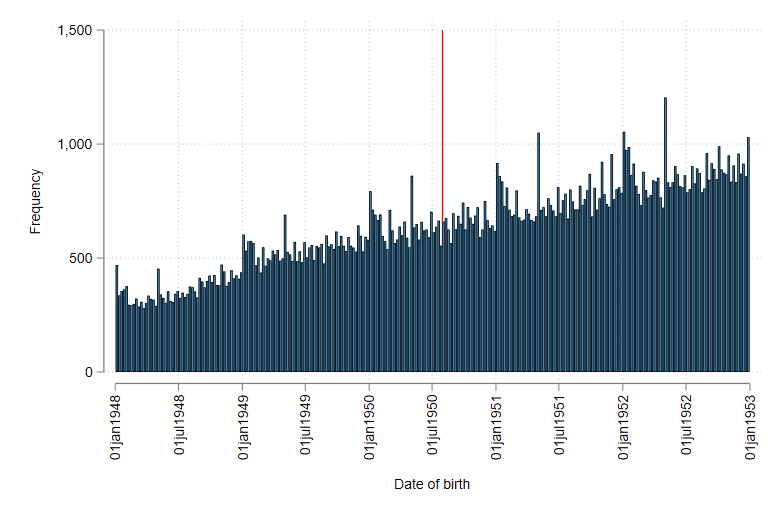
\includegraphics[width=\linewidth]{Graphs/hist_M50.png}
  \caption{M50 cohort}
\end{subfigure}%
\begin{subfigure}{.5\textwidth}
  \centering
  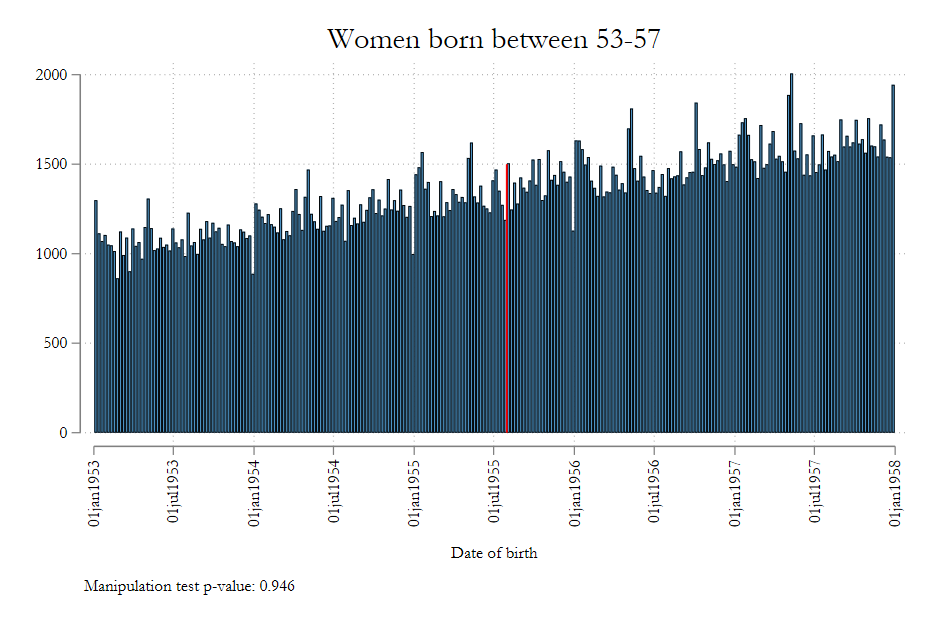
\includegraphics[width=\linewidth]{Graphs/hist_F55.png}
  \caption{F55 cohort}
\end{subfigure}
\fnote{\textit{Notes:} Panel (a) shows the distribution of birth dates for men born between 1948 and 1952. Panel (b) shows the distribution of birth dates for women born between 1953 and 1957. The red lines in each panel represent the cutoff date from LA-01. P-values from the McCrary density test are shown in the top left corner of each plot.}
\end{figure}

\begin{figure}[H]
\caption{Sample balance across cohorts}\label{fig:balance}
\centering 
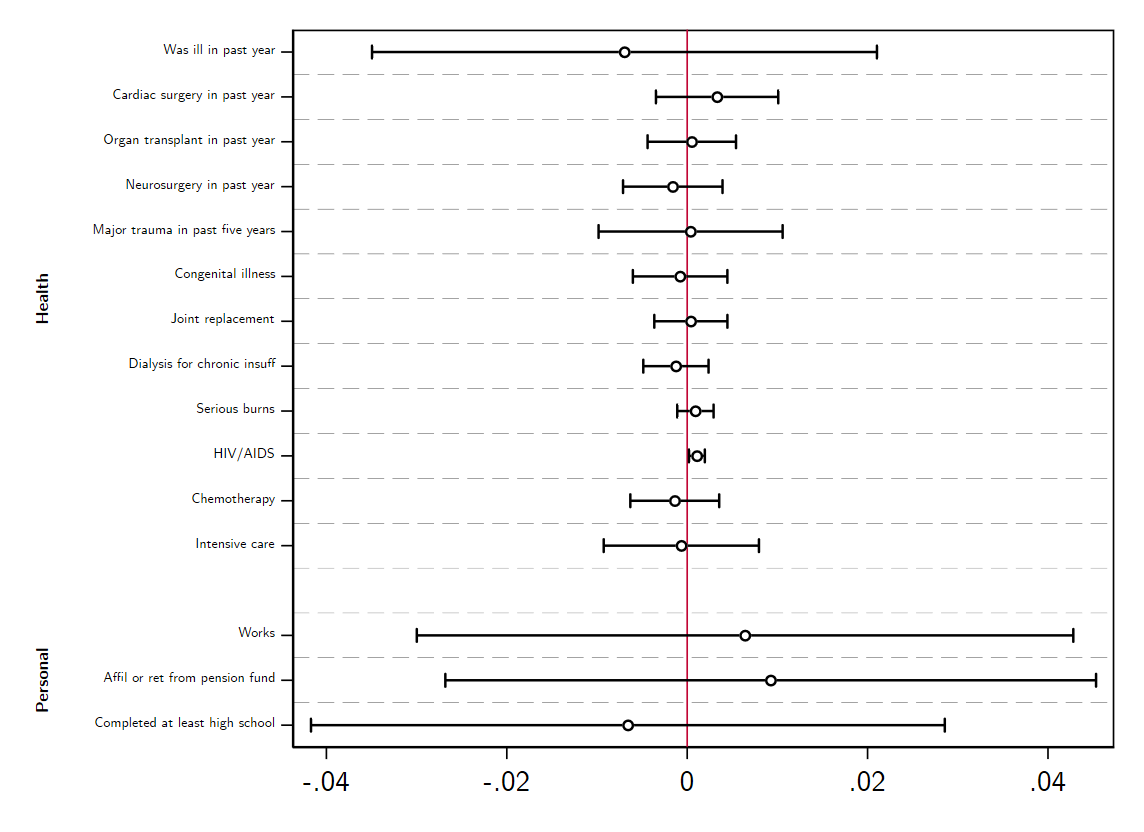
\includegraphics[width=\textwidth]{Graphs/balance_RD_final.png}
\fnote{\textit{Notes:} Each dot represents the point estimate from an RD regression. The lines across the coefficients are confidence intervals at the 95\% level. Regressions pool both cohorts and include cohort fixed effects.}
\end{figure}

\newpage
\section*{Tables}
}

\newpage
\bibliographystyle{apacite}
\bibliography{references}

\newpage
\appendix
\counterwithin{figure}{section}
\counterwithin{table}{section}

\section{Data construction appendix \label{sec:appdata}}

\end{document}